\documentclass[10pt, a4paper, titlepage, hidelinks]{article}
\usepackage{graphicx, latexsym}
\usepackage{setspace} 
\usepackage{apalike}
\usepackage{amssymb, amsmath, amsthm}
\usepackage{bm}
\usepackage{epstopdf}
\usepackage[]{hyperref}
\usepackage[
    backend = biber,
    style = apa,
    sorting = nyt,
    uniquename=false
    ]{biblatex}
\usepackage[margin=1.4in]{geometry}
\usepackage{microtype}
\usepackage{booktabs}
\usepackage{caption}
\usepackage{threeparttable}


\hypersetup{
    pdftitle={Transport Mode Detection in a Smartphone-based National Travel Survey},
    pdfauthor={Quinty Boer},
    pdfsubject={Research Report},
    pdfkeywords={},
    bookmarksnumbered=true,     
    bookmarksopen=true,         
    bookmarksopenlevel=1,       
    colorlinks=false,            
    pdfstartview=Fit,           
    pdfpagemode=UseOutlines,      
    pdfpagelayout=TwoPageRight
}

%\singlespacing
%\onehalfspacing
\doublespacing

\addbibresource{references.bib}
\addbibresource{references_additional.bib}

\title{Transport Mode Detection in a Smartphone-based National Travel Survey \\[0.5cm] \normalsize Research Report (Repurposed for Markup cCurse}
\author{Quinty Boer (4845242) \\ \normalsize \textit{Methodology and Statistics for the Behavioural, Biomedical and Social Sciences} \\[1cm] Advisors: \\ Yvonne A.P.M. Gootzen (CBS, TU/e) \\ Dr. Jonas Klingwort (CBS) \\ Dr. Peter Lugtig (UU) \\ Daniëlle Remmerswaal (UU) \\[1cm] FETC-approval: 24-1967 \\[1cm] \normalsize Candidate Journal: Transportation Research Interdisciplinary Perspectives \\[1cm] \normalsize Word count: 2494}
%\date{\today}
\date{}

\begin{document}
\maketitle
\newpage

\section{Introduction}


Understanding travel behaviour in a society is important for national infrastructure planning. Traditionally, information on travel behaviour is collected by national statistical institutes through diary surveys. In these types of surveys, respondents are asked to report in detail on all their trips over a period of time. Often, the requested information on travel behaviour includes the travel mode, time, duration, route, and purpose. Diary-based studies rely on the respondent's ability to remember their travel activities, which may be susceptible to under-reporting and response-over-time bias (\cite{mccool2021}; \cite{prelipcean2018}). Furthermore, these studies impose a high burden on the respondents, which is associated with an increased risk of non-response and dropout (\cite{wang2024}).

A proposed solution to the high-burden diary surveys is the use of smart surveys. In these surveys, data is collected by sensors available in smartphones. In the case of travel behaviour surveys, the passively collected sensor data can be used to gather information on individual travel behaviour (\cite{yang2018}). The collected geolocation measurements can be used to define segments consisting of trips and stops (\cite{safi2016}), which can then be used to compute statistics on the travel distance, speed, route, and duration. As a result, respondents are no longer required to manually record all the details of their trips, decreasing respondent burden considerably. Furthermore, sensor data may provide more detailed information on travel behaviour that is difficult to obtain from a diary survey, such as the average speed and the exact start and end times of trips (\cite{nahmias-biran2018}).

In 2018 and 2022/2023, Statistics Netherlands performed large-scale field tests of such an implementation of a smart survey in a travel app (\cite{Schouten2024}). A semi-automated approach was used in which the app automatically detects trips and stops, while respondents are asked to annotate these with information on the travel mode and stop purpose (\cite{zahroh2025}). Consequently, respondents may still experience the burden of remembering and providing details in the app. One way to further decrease respondent burden would be to automatically detect the transport mode, thereby eliminating the need for respondents to annotate their data. The aim of this research report is to share the preliminary findings of an exploratory study into the feasibility of using a machine learning model to automatically predict the travel mode.

The next section will briefly overview the current state of automatic transport mode detection and the most popular methods used. Section 3 contains information on the data and pre-processing steps, as well as a description of the methods used to create a preliminary random forest prediction model. After presenting the results, the discussion section will share some considerations and plans for future research.

\section{Background}

Most automatic transport mode detection methods can be separated into supervised and semi-supervised or unsupervised approaches. Whereas supervised learning algorithms require labeled data to train a prediction model, semi- and unsupervised learning algorithms are often suggested for sparsely labeled or non-labeled data (\cite{sadeghian2021}; \cite{yang2024}). As unlabeled data is typically easier and less expensive to obtain than labeled data, these algorithms are highly valuable in transportation research. However, as they are difficult to evaluate and do not allow for easy comparison (\cite{li2022}; \cite{markas&yu2020}), supervised algorithms are often preferred when labeled data is available.

Supervised learning approaches may be further separated into rule-based algorithms, traditional machine learning and deep learning. Rule-based algorithms have been successfully used to predict transport mode on GPS data and have the advantage of high interpretability (\cite{sadeghian2021}; \cite{xiao2019}). However, these approaches often see researchers manually adjusting decision rules, which may be time-intensive and requires expert knowledge (\cite{sadeghian2021}).

Although traditional machine learning models are typically less interpretable, they have been a popular choice for transport mode detection due to their high predictive performance (\cite{yang2024}). Some of the algorithms used in these models are support vector machines (SVM) (\cite{bolbol2012}), naive Bayes (NB) (\cite{nour2016}) and Bayesian networks (BN) (\cite{xiao2015}). Decision tree-based ensemble models like gradient-boosted trees and random forest are also commonly used (\cite{li2021}; \cite{lu2019}; \cite{shafique2016}; \cite{liu2022}). Out of these, the random forest model has been particularly popular, as it often outperforms other traditional supervised machine learning algorithms (\cite{bedogni2016}; \cite{bjerre-nielsen2020}; \cite{hasan2022}; \cite{sadeghian2022}). Considerable advantages of random forests are that they can handle high-dimensional data, require relatively little hyper-parameter tuning to train, and are less prone to over-fitting than many other machine learning methods (\cite{pappu2014}).

Finally, deep learning algorithms have the advantage of high flexibility in the model input. Whereas traditional supervised learning algorithms often require input on trip segment-level, deep learning algorithms allow for GPS measurement-level input. Creating features on a trip segment-level requires summarising and aggregating information from the GPS measurement-level to trip segment-level, resulting in information loss (\cite{yang2024}). Furthermore, deep learning algorithms such as Recurrent Neural Networks and Long Short-Term Memory have the additional advantage of automatically learning temporal patterns in the data ((\cite{jiang2023}; \cite{yu2021}; \cite{qin2019}). However, a large disadvantage of these algorithms is that they require a large quantity of high-quality data to be trained successfully, as well as high computational power. This project will therefore focus on traditional machine learning methods.

\section{Data and Methods}

\subsection{Data Collection and Pre-processing}

From November 2022 to February 2023, Statistics Netherlands collected smartphone sensor data from a sample of respondents from the general population as part of a field test of a smartphone travel app designed to measure travel behaviour in the Netherlands. The field test had an experimental design, where respondents were asked to use the travel app for one or seven days. Low-quality observations were removed from the data, including geolocation measurements with very low accuracy and respondents for which less than one hour of data was collected. Additionally, all duplicate measurements were removed from the data (\cite{Schouten2024}; \cite{gootzen2025}). 

After removing non-labeled trips, the remaining trip segment data consists of a total of 4219 labeled trips made by 252 users. Each trip segment has a start time, end time, and travel mode label that is one of either walking, bike, e-bike, car, bus, tram, metro, or train. The almost 3 million GPS data points that make up these trip segments consist of a timestamp, longitude, latitude, and accuracy value.

Information on the number of labeled trips for each transport mode class can be found in Table \ref{table:1}. Car trips occur most, followed by walking trips. The public transportation modes metro, tram, and bus occur least frequently in the data.

\subsection{Feature Engineering}

\begin{table}[]
        \caption{Labeled trips per transport mode class}
        \centering
        \resizebox{0.85\textwidth}{!}{%
        \begin{tabular}{lcccccccc}
        \toprule
        & Car & Bus & E-Bike & Bike & Metro & Tram & Train & Walking \\
        \midrule
        & 1881 & 95 & 146 & 821 & 56 & 34 & 157 & 1029 \\
        \bottomrule
        \label{table:1}
        \end{tabular}
        }
    \end{table}

%Features were created as input for a machine learning model in two steps.
First, features were calculated on the GPS measurement-level. The Haversine formula for great-circle distance between two points was used to determine the distance traveled between two consecutive GPS measurements. The distance traveled and the time difference between points were then used to calculate speed and its higher-order derivatives acceleration, jerk, and snap. Acceleration measures the rate of change of speed, jerk measures the rate of change of acceleration, and snap measures the rate of change of jerk. Additionally, bearing was calculated based on the difference in longitude and latitude between two points. The bearing was only calculated for GPS measurements corresponding with a speed of at least 0.6 m/s. Calculating the bearing for GPS measurements with a lower speed resulted in highly diverging consecutive bearing values that were deemed uninformative. All calculations were performed with the \texttt{geosphere} package in R (\cite{geosphere}; \cite{R}).

In the second step, GPS-level features were aggregated to the trip segment-level by summarising the GPS-based features for all data points between the trip segment's start and end time. Additionally, the accuracy of GPS measurements, frequency of measurement gaps (more than 5 minutes between consecutive timestamps), and frequency and size of outliers and implausible values were taken into account. Lastly, features such as day of the week, time of day, and whether the trip was made during rush hour were added to the model.

\subsection{Modeling}

The preliminary model is a random forest classifier based on the features calculated from the GPS data described previously. As preparation, the data was split into training data and testing data using a 70/30 split ratio. A blocking strategy was used to ensure that all trip segments belonging to a single respondent are either included in the training or testing data. This strategy should prevent overly optimistic predictions when potentially similar trips from a single respondent are used for both training and testing the model.

A random forest prediction model was created with the \texttt{ranger} package in R, using the streamlining functions included in the \texttt{caret} package (\cite{ranger}; \cite{caret}). Model hyper-parameters were tuned using 10-fold cross-validation on the training data. The same type of blocking strategy that was used for splitting the train and test data was used for the creating the folds. The number of decision trees in the random forest model was set to 50 trees and 54 features were considered by each tree when splitting a node.

\subsection{Evaluation}

The model performance is measured with the balanced accuracy and F1 score of the test data for each of the transport modes. Both evaluation criteria are confusion matrix-based metrics that are suitable for multi-class classification in imbalanced datasets (\cite{luque2019}). Whereas the balanced accuracy is the mean of the true positive rate (recall) and the true negative rate, the F1 score balances the precision or positive predictive value with the recall. F1 scores close to 1 indicate high precision and recall, whereas scores below 0.5 indicate a poor prediction performance.

The F1 Score is the harmonic mean of precision and recall:
\begin{align*}
F_1 &= 2 \cdot \frac{\text{Precision} \cdot \text{Recall}}{\text{Precision} + \text{Recall}}
\end{align*}

The balanced accuracy is the average of recall for each class:
\begin{align*}
\text{Balanced Accuracy} &= \frac{1}{C} \sum_{i=1}^{C} \frac{\text{TP}_i}{\text{TP}_i + \text{FN}_i}
\end{align*}
\begin{center}
where $C$ is the number of classes.
\end{center}

Additionally, feature importance in the random forest model is evaluated using the permutation variable importance measure (\cite{altmann2010}). This measure can be understood as the mean decrease in prediction accuracy and can be calculated by looking at the decrease in accuracy when the values on one feature are randomly shuffled, thereby isolating the effect of that particular feature on the model's prediction performance. This method is often preferred over the default impurity or Gini importance measure (\cite{janitza2018}).

\section{Preliminary Results}

\subsection{Prediction Performance}

The model's prediction performance on the test data is summarised in the confusion matrix and evaluation criteria overview in Tables 2 and 3. Both tables highlight considerable differences in prediction performance across transport modes. The overrepresented classes walking, car, and bike are often classified correctly, achieving F1 scores of 0.88, 0.87, and 0.79 respectively. The model performed moderately well on train trips, with some misclassification into car trips and an F1 score of 0.75.

Contrastingly, the model did not perform well on the underrepresented classes bus, metro, tram, and e-bike. Bus and tram trips were consistently misclassified as car trips, while metro trips were also misclassified as walking trips. Furthermore, over 60\% of e-bike trips were misclassified as bike trips. F1 scores for these transport modes are all below 0.2. Bus and tram received F1 scores of 0, as these were never correctly classified.

\begin{table}[]
        \centering
        %\caption{\parbox{0.75\textwidth}{\centering Table 2: Confusion matrix comparing observed and predicted transport modes in the test data}}
        \caption*{\centering\begin{minipage}{0.75\textwidth}Table 2: Confusion matrix comparing observed and predicted transport modes in the test data \end{minipage}}
        \resizebox{0.75\textwidth}{!}{%
        \begin{tabular}{lcccccccc}
        \toprule
        \textbf{} & \multicolumn{8}{c}{\textbf{Observed}} \\
        \cmidrule(lr){2-9}
        \textbf{Predicted} & Car & Bus & E-bike & Bike & Metro & Tram & Train & Walking \\
        \midrule
        Car     & \textbf{472} & 33 & 4 & 30 & 11 & 8 & 8 & 19 \\
        Bus     & 1 & \textbf{0} & 0 & 3 & 1 & 1 & 0 & 0 \\
        E-bike  & 1 & 0 & \textbf{3} & 10 & 0 & 0 & 0 & 0 \\
        Bike    & 4 & 0 & 11 & \textbf{170} & 0 & 1 & 0 & 19 \\
        Metro   & 0 & 0 & 0 & 0 & \textbf{1} & 0 & 0 & 0 \\
        Tram    & 1 & 0 & 0 & 0 & 0 & \textbf{0} & 0 & 0 \\
        Train   & 9 & 0 & 0 & 1 & 3 & 0 & \textbf{31} & 0 \\
        Walking & 17 & 0 & 0 & 13 & 8 & 0 & 0 & \textbf{279} \\
        \bottomrule
        \label{table:2}
        \end{tabular}%
        }
    \end{table}

    \begin{table}[]
        \centering
        \caption*{\centering\begin{minipage}{0.75\textwidth}Table 3: F1 scores and accuracy per class in the test data. High values indicate good predictive performance \end{minipage}}
        \resizebox{0.75\textwidth}{!}{%
        \begin{tabular}{lcccccccc}
        \toprule
        & Car & Bus & E-bike & Bike & Metro & Tram & Train & Walking \\
        \midrule
        F1 score & 0.87 & 0 & 0.19 & 0.79 & 0.08 & 0 & 0.75 & 0.88 \\
        Accuracy & 0.88 & 0.50 & 0.58 & 0.86 & 0.52 & 0.50 & 0.89 & 0.92 \\
        \bottomrule
        \label{table:3}
        \end{tabular}%
        }
    \end{table}


\subsection{Feature Importance}

Feature importance analysis revealed that speed-related features were the most important predictors in the random forest model, as they collectively represent the top 8 most influential features. The top 10 most important features out of 114 features included in the model are provided in Figure 1.

The important speed-related features describe the central tendency and variability of a trip's speed, such as the overall mean/median and the mean/median speed when a person is in motion, the standard deviation and the inter-quartile range. The most influential feature is speed at the 90th percentile, which represents the value below which 90\% of the GPS data points in a trip fall. It can be interpreted as the speed value that separates the highest 10\% of speed observations during a trip.

The importance of speed-related features aligns with the model's performance in distinguishing walking, car, and bike trips, which tend to have distinct speed patterns. However, it may also partially explain the poor prediction performance for e-bike, tram, and bus. These transport modes may have speed characteristics that are difficult to distinguish from bike and car trips. As they are also underrepresented in the data, it may be difficult for a machine learning model to learn the unique speed patterns associated with these transport modes.

\begin{figure}
    \centering
    \caption{Feature importance of the 10 most important features}
    \vspace{-0.5cm}
    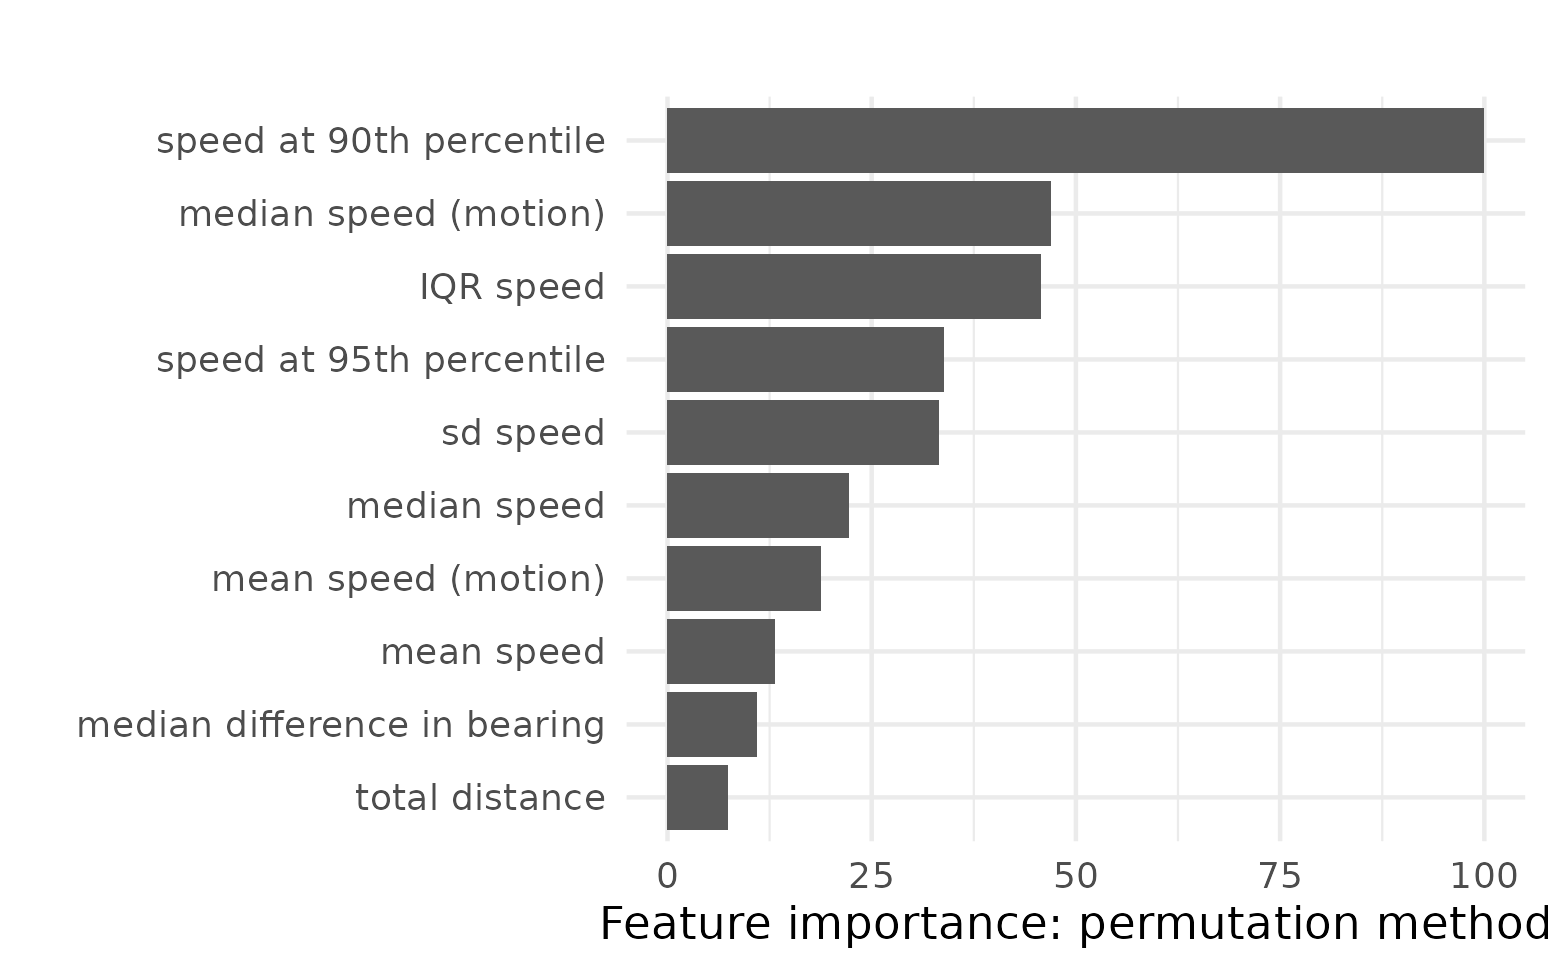
\includegraphics[width=0.9\textwidth]{varimp_plot.png}
    \end{figure}

\section{Discussion}

In this preliminary random forest model, sensor data collected in a travel app were used to create features to predict the transport mode of trips made by respondents. The reported findings are meant to serve as a baseline for further research to see whether prediction performance can be increased by adding additional data sources and accounting for temporal dependencies. While the preliminary random forest model is able to predict common transport modes such as car, bike, and walking relatively well, it struggles to classify the underrepresented transport modes such as bus, tram, and metro. This discussion will outline some considerations and steps to be taken in the remainder of this project.

\subsection{Additional Data Sources}

First, additional features will be created that incorporate geospatial information using OpenStreetMap (OSM) data. Researchers have previously incorporated geospatial information into their transport mode detection models by creating features such as the proximity to public transport stations and public transport network lines (\cite{liu2022}; \cite{li2021}; \cite{nour2016}). Adding features based on geospatial information from an external source like OSM is expected to help in distinguishing between public transport modes and non-public transport modes that share similar speed characteristics.

%Second, it will be explored whether making use of a combination of random up-sampling and down-sampling in the training data will help reduce potential issues for the random forest model caused by class imbalances. As random up-sampling may increase the risk of over-fitting and random down-sampling results in a loss of information, a combination of these two strategies might improve the model slightly.

\subsection{Accounting for Temporal Dependencies}

Random forest models assume that observations are independent and do not automatically account for potential temporal dependencies between observations (\cite{hu&szymczak2023}; \cite{sela&simonoff2020}). As the data in this project contains multiple trips made by individuals over a time period, it may be worth exploring whether we can account for potential temporal dependencies between trips by adding lagged features. Lagged features contain information on previous trips made at earlier time points. Information may include the (predicted) transport mode of previous trips, but also the time between consecutive trips and whether previous trips were made during a similar time of day. For the current test data, the information on previous trips is available and can be used directly as input for the features. However, as this information will not be available for unlabeled future data, transport mode prediction will become an iterative process with earlier predictions serving as input to help predict future trips.

\subsection{Generalisability}

When a machine learning model is trained on data situated in a specific time and context and used to make predictions on unseen future data, there may be concerns about the generalisability of the trained model. This concern may be relevant for the preliminary model that has been created, as well as for future models that are trained on the same data. As the data was collected exclusively during the winter of 22/23, we do not know whether the model may be biased toward seasonal travel patterns caused by differences in weather or events. Travel behaviour of individuals may differ considerably depending on the season. This may especially be an issue for the transport modes that are underrepresented in the data, as the risk of issues with extrapolation tends to be larger for these classes. Potentially testing the model on travel behaviour data collected in a different time period may provide some insights into whether generalisability will be a large concern.

\newpage

\microtypesetup{protrusion=false}

\printbibliography[title = {References}]

\end{document}



